\documentclass[11pt,a4paper]{jsarticle}

%%%%%%%%%%%%%%%%%%%%%%%%%
% Packages
%%%%%%%%%%%%%%%%%%%%%%%%%
\usepackage{
	amsmath, % 環境
	amssymb, % 記号
	amsfonts % 特殊文字
}
\usepackage{ascmac}
\usepackage{ulem}
\usepackage{lmodern}
\usepackage{bm}
\usepackage{mathtools, centernot, physics}
\usepackage{enumerate}
% \usepackage{graphicx}
\usepackage[dvipdfmx]{graphicx}
\usepackage{comment} % 複数行をコメントアウトする
\usepackage{url}
\usepackage{array, booktabs, multirow, makecell} % tabular関連
% \usepackage{romannum} % ローマ数字
% \usepackage{xcolor}
\usepackage[dvipdfmx, dvipsnames]{xcolor}
\usepackage{setspace}
\usepackage{float}

%%%%%%%%%%%%%%%%%%%%%%%%%
% Format
%%%%%%%%%%%%%%%%%%%%%%%%%
\setlength{\textwidth}{\fullwidth}
\setlength{\textheight}{40\baselineskip}
\addtolength{\textheight}{\topskip}
\setlength{\voffset}{-0.2in}
\setlength{\topmargin}{0pt}
\setlength{\headheight}{0pt}
\setlength{\headsep}{0pt}

%%%%%%%%%%%%%%%%%%%%%%%%%
% Definitions
%%%%%%%%%%%%%%%%%%%%%%%%%
\newcommand{\alert}[1]{\textbf{\textcolor{red}{#1}}}
\newcommand{\rainn}{\textcolor{blue}{\uline{\ \ \ \ }}}
\newcommand{\sizi}[1]{\textcolor{OliveGreen}{\lbrack #1\rbrack}}

	
\begin{document}
\section{目的}
抵抗素子および容量素子を用いて構成される積分回路(低域通過型フィルタ)の特性を実験により確認し、
その動作を理解する。

\section{原理}
はじめに本実験で用いるRC回路図を示す。
\begin{figure}[H]
    \centering
    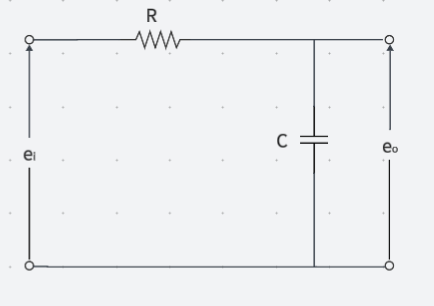
\includegraphics[width=0.8\linewidth]{rc.png}
    \caption{RC積分回路}
    \label{fig:rc}
\end{figure}

RC積分回路は抵抗およびコンデンサから構成される回路であり、
低周波成分を通過させ、高周波成分を減衰させる低域通過型フィルタ（LPF）として動作する。

正弦波を入力した場合の積分回路の伝達関数は、
\begin{equation}
\frac{E_o}{E_i}
=
\frac{1}{1+j\omega RC}
\end{equation}
で表される。ここで、$E_i$は入力電圧、$E_o$は出力電圧、$\omega$は角周波数を示す。

伝達関数の振幅特性は、
\begin{equation}
\left|\frac{E_o}{E_i}\right|
=
\frac{1}{\sqrt{1+(\omega RC)^2}}
\end{equation}
となる。この式より、低周波領域では出力電圧は入力電圧とほぼ等しくなり、
高周波領域では出力電圧が減衰する。

また、位相特性は、
\begin{equation}
\phi
=
-\tan^{-1}(\omega RC)
\end{equation}
で表され、出力電圧は入力電圧に対して遅れる。

積分回路の遮断周波数$f_c$は、
\begin{equation}
f_c
=
\frac{1}{2\pi RC}
\end{equation}
で与えられる。この周波数において、出力電圧は入力電圧の$1/\sqrt{2}$倍となり、
利得は$-3$ dBとなる。

一方、ステップ電圧を入力した場合、コンデンサの充電に伴い出力電圧は時間とともに増加し、その時間応答は、
\begin{equation}
e_o
=
E\left(1-e^{-t/RC}\right)
\end{equation}
で表される。ここで、時定数$\tau$は、
\begin{equation}
\tau=RC
\end{equation}
であり、回路の応答速度を決定する重要なパラメータである。


\section{方法}

\subsection{RC回路の周波数特性}
使用した抵抗およびコンデンサはテスターで測定し、抵抗値は$2.989\,\mathrm{k\Omega}$,
コンデンサ容量は$0.00992\,\mathrm{\mu F}$であった。
以下に作成したRC積分回路の配線を示す。

\begin{figure}[H]
    \centering
    \includegraphics[width=0.8\linewidth]{回路図.png}
    \caption{RC積分回路の配線}
    \label{fig:rc_lpf}
\end{figure}


図\ref{fig:rc_lpf}の回路に対し、
発振器から正弦波を入力した。周波数を10Hzから1MHzまで変化させた。なお、測定に先立ち、
使用した抵抗値およびコンデンサ容量から遮断周波数$f_c$を計算し、測定周波数の一つとした。
電圧計を用いて入力電圧$E_i$および出力電圧$E_o$を測定し、
\begin{equation}
G=20\log_{10}\left(\frac{E_o}{E_i}\right)
\end{equation}
より利得を求めた。また、オシロスコープを用いて入力波形と出力波形の時間差$\Delta t$を測定し、
\begin{equation}
\phi =360\frac{\Delta t}{T}
\end{equation}
より位相差を算出した。

\subsection{RC回路の時定数の測定}

周波数特性の測定で作製したRC積分回路について、抵抗値を
$2.989\,\mathrm{k\Omega}$および$10.00\,\mathrm{k\Omega}$とし、
コンデンサ容量$0.00992\,\mathrm{\mu F}$を用いて時定数の測定を行った。
以下に時定数測定に用いたRC積分回路の配線を示す。

\begin{figure}[H]
    \centering
    \includegraphics[width=0.8\linewidth]{tau.png}
    \caption{時定数測定に用いたRC積分回路の配線}
    \label{fig:au}
\end{figure}

図\ref{fig:au}の回路に方形波を入力した。方形波の周期は出力波形が十分に定常状態へ達するように、
$T>10RC$となるよう設定した。

入力波形および出力波形をオシロスコープで観測し、両波形の立ち上がり位置がほぼ一致するように調整した。
その後、あらかじめ計算した理論値の時定数$\tau$を参考に、オシロスコープの時間軸を調整しながら、
カーソル機能を用いて出力波形が入力波形と概ね一致し始める位置を決定した。最後に、もう一方のカーソルを
入力波形の立ち上がり位置に合わせ、2つのカーソル間の時間差を測定した。

\section{実験結果}
\subsection{RC回路の周波数特性}

式(4)より、使用した抵抗値$R=2.989\,\mathrm{k\Omega}$およびコンデンサ容量
$C=0.00992\,\mathrm{\mu F}$から遮断周波数$f_c$を計算すると、

\begin{equation}
f_c
=
\frac{1}{2\pi RC}
=
5367\,\mathrm{Hz}
\end{equation}

となった。
以下に$f_c$における波形を示す。ただし、CH1が入力波形、CH2が出力波形である。
\begin{figure}[H]
    \centering
    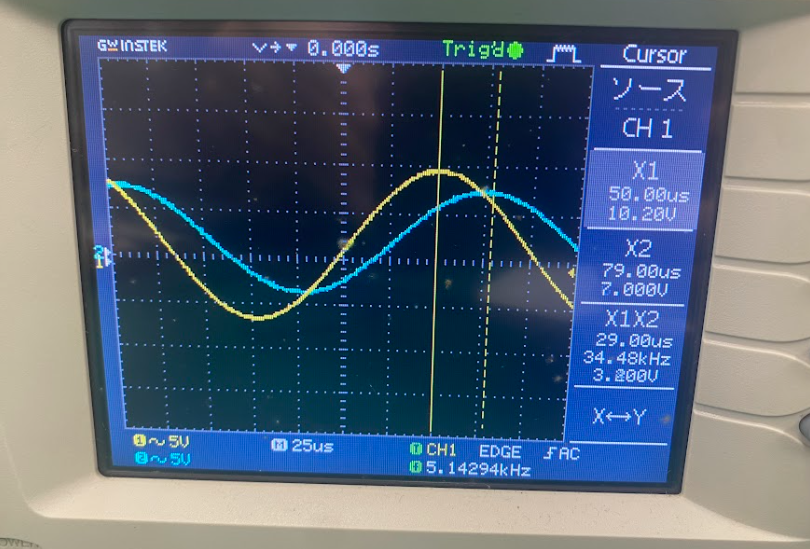
\includegraphics[width=0.8\linewidth]{fc.png}
    \caption{遮断周波数$f_c$における波形}
    \label{fig:fc}
\end{figure}

また、表1に測定結果および理論値を示す。
\begin{table}[H]
\centering
\caption{RC積分回路の周波数特性の測定結果および理論値}
\label{tab:freq}
\small
\begin{tabular}{ccccccccc}
\toprule
$f$ & $E_i$ & $E_o$ & $\Delta t$ & $T$
& 利得 & 位相差 & 理論利得 & 理論位相 \\
(Hz)&(V)&(V)&(s)&(s)&(dB)&($^\circ$)&(dB)&($^\circ$)\\
\midrule
10      &0.100&0.100&0                &0.1000& 0.00 &  0.0&  0.00& -0.11\\
100     &0.100&0.100&0                &0.0100& 0.00 &  0.0&  0.00& -1.07\\
1000    &0.100&0.100&$-6.0\times10^{-5}$&0.0010& 0.00 &-21.6& -0.15&-10.55\\
5367    &0.550&0.390&$-2.9\times10^{-5}$&$1.86\times10^{-4}$&-2.99&-56.0&-3.01&-45.00\\
10000   &0.100&0.0410&$-1.8\times10^{-5}$&$1.00\times10^{-4}$&-7.74&-64.8&-6.50&-61.77\\
100000  &4.99 &0.280&$-2.4\times10^{-6}$&$1.00\times10^{-5}$&-25.02&-86.4&-25.42&-86.93\\
1000000 &2.65 &0.0125&$-2.5\times10^{-7}$&$1.00\times10^{-6}$&-46.53&-90.0&-45.40&-89.69\\
\bottomrule
\end{tabular}
\end{table}


\subsection{RC回路の時定数の測定}

抵抗値$R=2.989\,\mathrm{k\Omega}$およびコンデンサ容量
$C=0.00992\,\mathrm{\mu F}$を用いた場合、理論値の時定数は

\begin{equation}
\tau=RC
=(2.989\times10^3)(0.00992\times10^{-6})
=29.65\,\mathrm{\mu s}
\end{equation}

となる。方形波の周期は$T>10RC$となるように設定するため、

\begin{equation}
T>296.5\,\mathrm{\mu s}
\end{equation}

となり、入力周波数は

\begin{equation}
f<\frac{1}{296.5\times10^{-6}}
=3372\,\mathrm{Hz}
\end{equation}

を満たす必要がある。したがって、本実験では$f=3\,\mathrm{kHz}$を用いた。

同様に、抵抗値$R=10.00\,\mathrm{k\Omega}$の場合、

\begin{equation}
\tau=99.20\,\mathrm{\mu s}
\end{equation}

であり、

\begin{equation}
T>992\,\mathrm{\mu s}
\end{equation}

となるため、

\begin{equation}
f<1008\,\mathrm{Hz}
\end{equation}

を満たす必要がある。したがって、本実験では$f=300\,\mathrm{Hz}$を用いた。
表2に測定結果および理論値を示す。
\begin{table}[H]
\centering
\caption{時定数の測定結果}
\label{tab:tau}
\begin{tabular}{ccccc}
\toprule
$R$ [$\mathrm{k\Omega}$] &
$f$ [Hz] &
理論値$\tau$ [$\mathrm{\mu s}$] &
縮尺 [$\mathrm{\mu s/div}$] &
実測値$\tau$ [$\mathrm{\mu s}$] \\
\midrule
2.989 & 3000 & 29.65 & 10 & 27.60\\
10.00 & 300  & 99.20 & 100 & 89.00\\
\bottomrule
\end{tabular}
\end{table}


\section{考察}
\subsection{RC回路の周波数特性}
表\ref{tab:error}に測定結果と理論値の絶対誤差を示す。
\begin{table}[H]
\centering
\caption{測定値と理論値の誤差}
\label{tab:error}
\small
\begin{tabular}{ccc}
\toprule
$f$ [Hz]
&
利得誤差 [dB]
&
位相誤差 [$^\circ$]
\\
\midrule
10      &0.00&0.11\\
100     &0.00&1.07\\
1000    &0.15&11.05\\
5367    &0.02&11.03\\
10000   &1.24&3.03\\
100000  &0.40&0.53\\
1000000 &1.12&0.31\\
\bottomrule
\end{tabular}
\end{table}
次に、図\ref{fig:ritoku}および図\ref{fig:isou}に、RC積分回路の利得および位相の周波数特性を示す。

\begin{figure}[H]
\centering
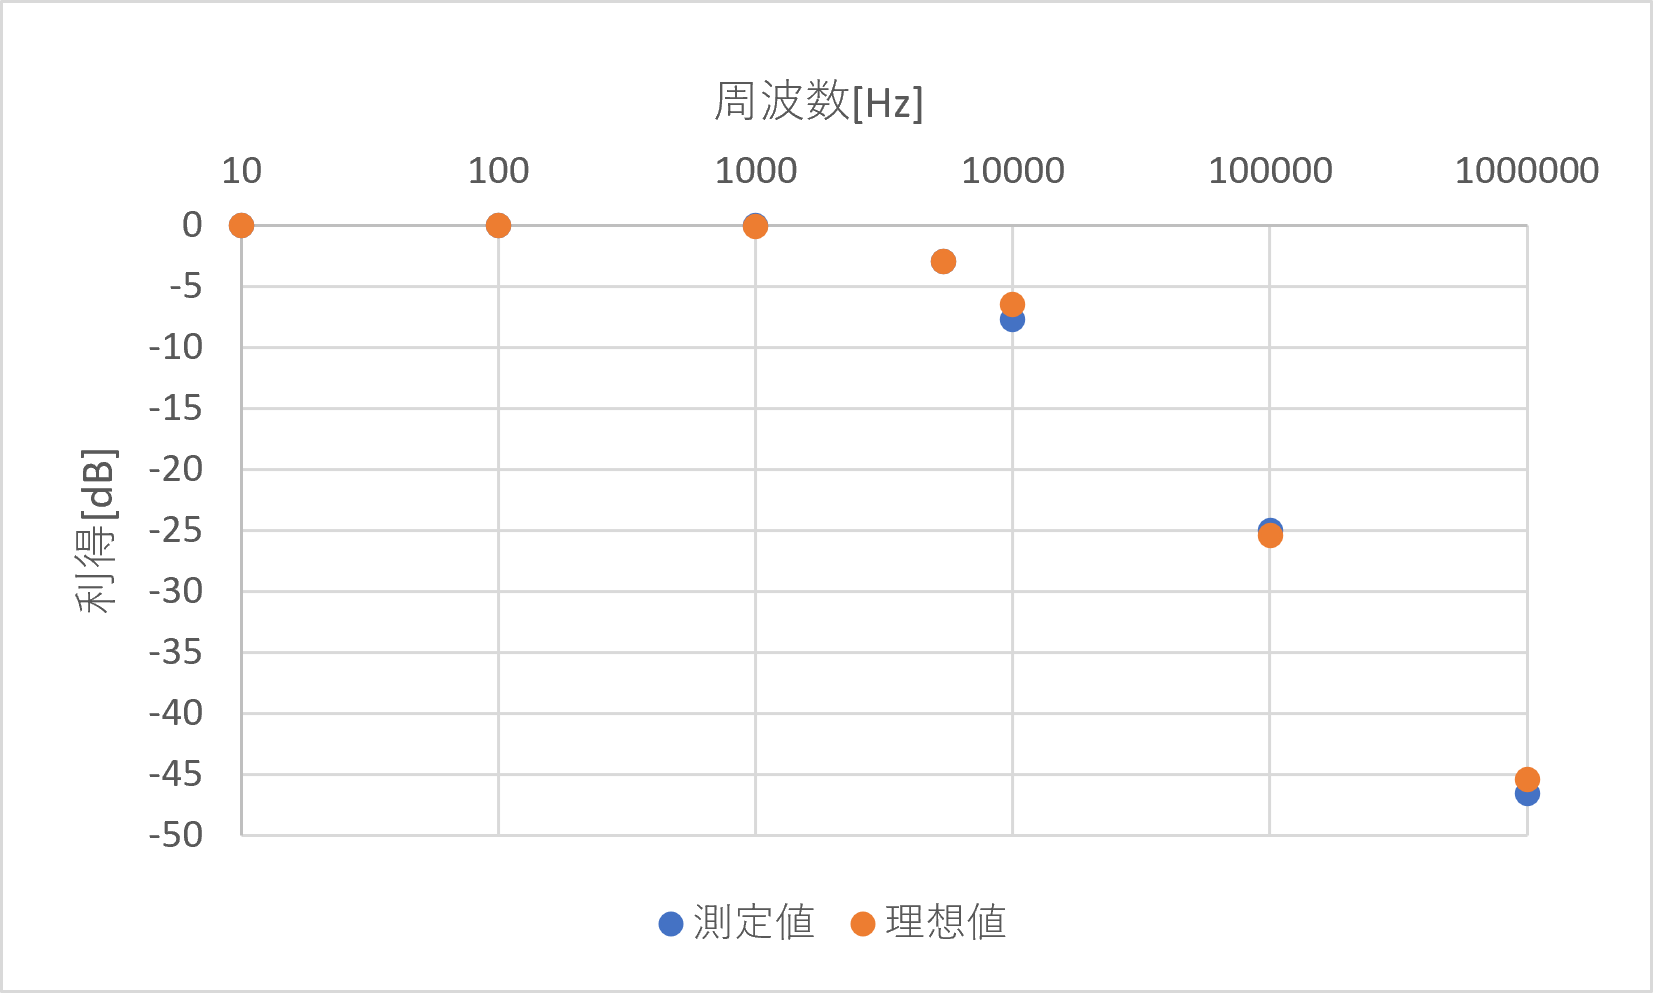
\includegraphics[width=0.8\textwidth]{ritoku.png}
\caption{RC積分回路の利得周波数特性（測定値および理論値）}
\label{fig:ritoku}
\end{figure}

\begin{figure}[H]
\centering
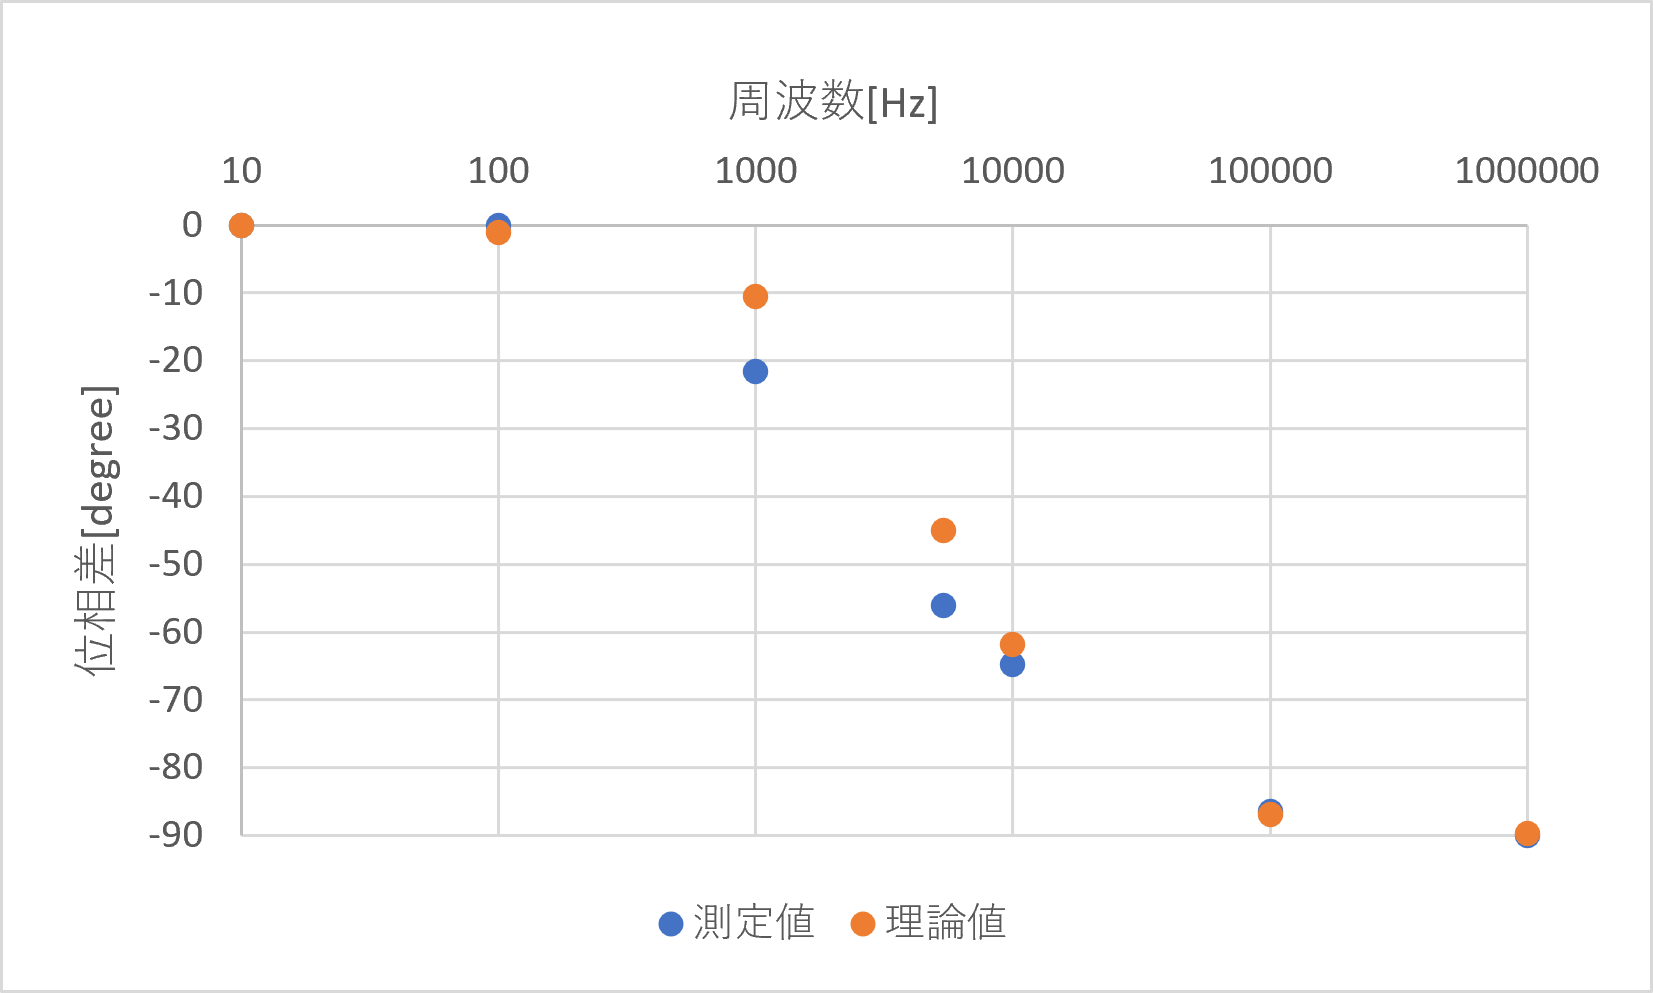
\includegraphics[width=0.8\textwidth]{isou.png}
\caption{RC積分回路の位相周波数特性（測定値および理論値）}
\label{fig:isou}
\end{figure}


表\ref{tab:error}より、利得は全周波数帯域で理論値と概ね一致していることがわかる。
一方、位相差については1000Hzおよび遮断周波数付近で比較的大きな差が見られた。
特に、1000Hzでは11.05$^\circ$、遮断周波数では11.03$^\circ$の誤差が生じた。
1000Hzおよび遮断周波数付近では、位相特性の傾きが大きく、周波数に対して位相差が急激に変化する領域である。
そのため、オシロスコープ上での時間差$\Delta t$のわずかな読み取り誤差が位相差に大きく影響し、
他の周波数帯域と比較して大きな誤差が生じたと考えられる。一方、低周波および高周波領域では位相差の変化が
緩やかであるため、読み取り誤差による影響は比較的小さかったと考えられる。


遮断周波数$f_c=5367\,\mathrm{Hz}$における利得は、測定値が$-2.99\,\mathrm{dB}$、理論値が$-3.01\,\mathrm{dB}$となり、両者はよく一致した。これは、遮断周波数において出力電圧の振幅が入力電圧の約$1/\sqrt{2}$倍となるという理論と一致している。また、位相については出力波形が入力波形に対して遅れていることが確認でき、RC積分回路が低域通過フィルタとして動作していることが確認できた。

\subsection{RC回路の時定数の測定}
表\ref{tab:tau_error}に時定数の理論値と実測値の比較を示す。
\begin{table}[H]
\centering
\caption{時定数の理論値と実測値の比較}
\label{tab:tau_error}
\begin{tabular}{ccccc}
\toprule
$R$ [k$\Omega$] &
$f$ [Hz] &
理論値$\tau$ [$\mu$s] &
実測値$\tau$ [$\mu$s] &
誤差[\%] \\
\midrule
2.989 & 3000 & 29.65 & 27.60 & 6.91 \\
10.00 & 300 & 99.20 & 89.00 & 10.28 \\
\bottomrule
\end{tabular}
\end{table}

時定数の誤差要因として、発振器の内部抵抗$r$の影響を考える。
図に発振器内部抵抗を考慮したRC積分回路を示す。
\begin{figure}[H]
    \centering
    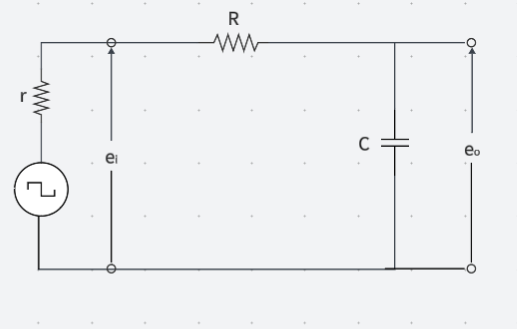
\includegraphics[width=0.8\linewidth]{r.png}
    \caption{発振器の内部抵抗を考慮したRC積分回路}
    \label{fig:r}
\end{figure}
積分回路において発振器の内部抵抗$r$を考慮すると、出力電圧のラプラス変換は、

\begin{equation}
E_o(s)
=
\frac{\frac{1}{sC}}{(r+R)+\frac{1}{sC}}
\frac{E}{s}
\end{equation}

と表される。これを整理すると、

\begin{equation}
E_o(s)
=
\frac{E}{s}
-
\frac{E}{s+\frac{1}{C(r+R)}}
\end{equation}

となる。したがって、逆ラプラス変換より、

\begin{equation}
e_o(t)
=
E\left(1-e^{-\frac{t}{C(r+R)}}\right)
\end{equation}

が得られる。通常のステップ応答

\begin{equation}
e_o(t)
=
E\left(1-e^{-\frac{t}{\tau}}\right)
\end{equation}

と比較すると、内部抵抗を考慮した時定数は、

\begin{equation}
\tau'
=
C(r+R)
\end{equation}

となる。

したがって、発振器の内部抵抗を考慮すると時定数は理論値より大きくなることが分かる。
しかし、本実験では実測値は理論値より小さい値となったため、発振器の内部抵抗のみでは
今回の誤差を説明することはできない。

本実験では、出力波形が入力波形と概ね重なり始める位置を目安として時定数を測定したため、
その位置の判断に主観が入ることが誤差の一因であると考えられる。また、オシロスコープのカーソル位置の
設定や時間軸の調整に伴う時間読取り誤差も測定結果に影響を与えたものと考えられる。

\section{参考文献}

\begin{enumerate}
\renewcommand{\labelenumi}{[\arabic{enumi}]}

\item 2026年度アナログ回路実験テキスト，第1回「RC回路の特性」.

\end{enumerate}

\end{document}